As the number of news articles published each day grows, it becomes impossible to manually examine them all to learn about events happening in the world. The field of Event Detection arose as a subfield of Information Retrieval \citep{information-retrieval-2, information-retrieval} and Topic Detection and Tracking \citep{tdt, tdt-2} with a goal to aid the users by automatically discovering important events in document collections.

More precisely, given a stream of text documents published over a certain time period, the task is to analyze them and output a collection of events that happened in the world during the period. An event is loosely defined as \textit{something happening in a certain place at a certain time} \citep{retrospective-online-study}.

In this thesis, we chose to modify an approach introduced by \cite{event-detection}, which is a retrospective \footnote{Discussed in \autoref{sec:related-event-detection}} method relying on event representation through keywords. We build upon this method to incorporate a more advanced way of measuring semantic similarity between words, as well as propose an alternative algorithm for the event detection itself. Furthermore, we use the results to generate a more human-readable event representation than a simple set of keywords.

The rest of the thesis is organized as follows. First, in \autoref{chap:related-work}, we are going to discuss related work. Then, in \autoref{chap:data-preprocessing}, we describe the document collection used for evaluation and the preprocessing steps taken.

In \autoref{chap:word-analysis}, we describe the original paper's procedure used to extract temporal characteristics of the individual words. These characteristics are then examined to reveal a subset of words which may be related to certain events, as opposed to generally appearing noisy words, so called \textit{stopwords}. Then, we will proceed to the event detection itself.

In the original paper, the semantic similarity between two words is computed in only a simple manner in terms of their document overlap. We replace this coarse measure by applying the recent advances in word embeddings, hopefully obtaining a finer measure of word similarity. This will be more discussed in \autoref{chap:event-detection}.

Although a set of related keywords provides a concise event representation, it is not particularly readable to the user. In \autoref{chap:document-retrieval}, we follow by interpreting each keyword set as a query to the document collection. This allows us to employ information retrieval techniques to obtain documents relevant to each event.

Since the number of documents may be still too high, we also generate a short annotation for each event. The user can quickly skim through these annotations to get an idea what the events are about, and decide which of them are worth a closer examination. This will be addressed in \autoref{chap:event-annotation}.

Finally, we evaluate our method and compare it to the original paper in \autoref{chap:evaluation}. We then conclude the thesis in \autoref{chap:conclusion}.

\begin{figure}[H]
  \centering
  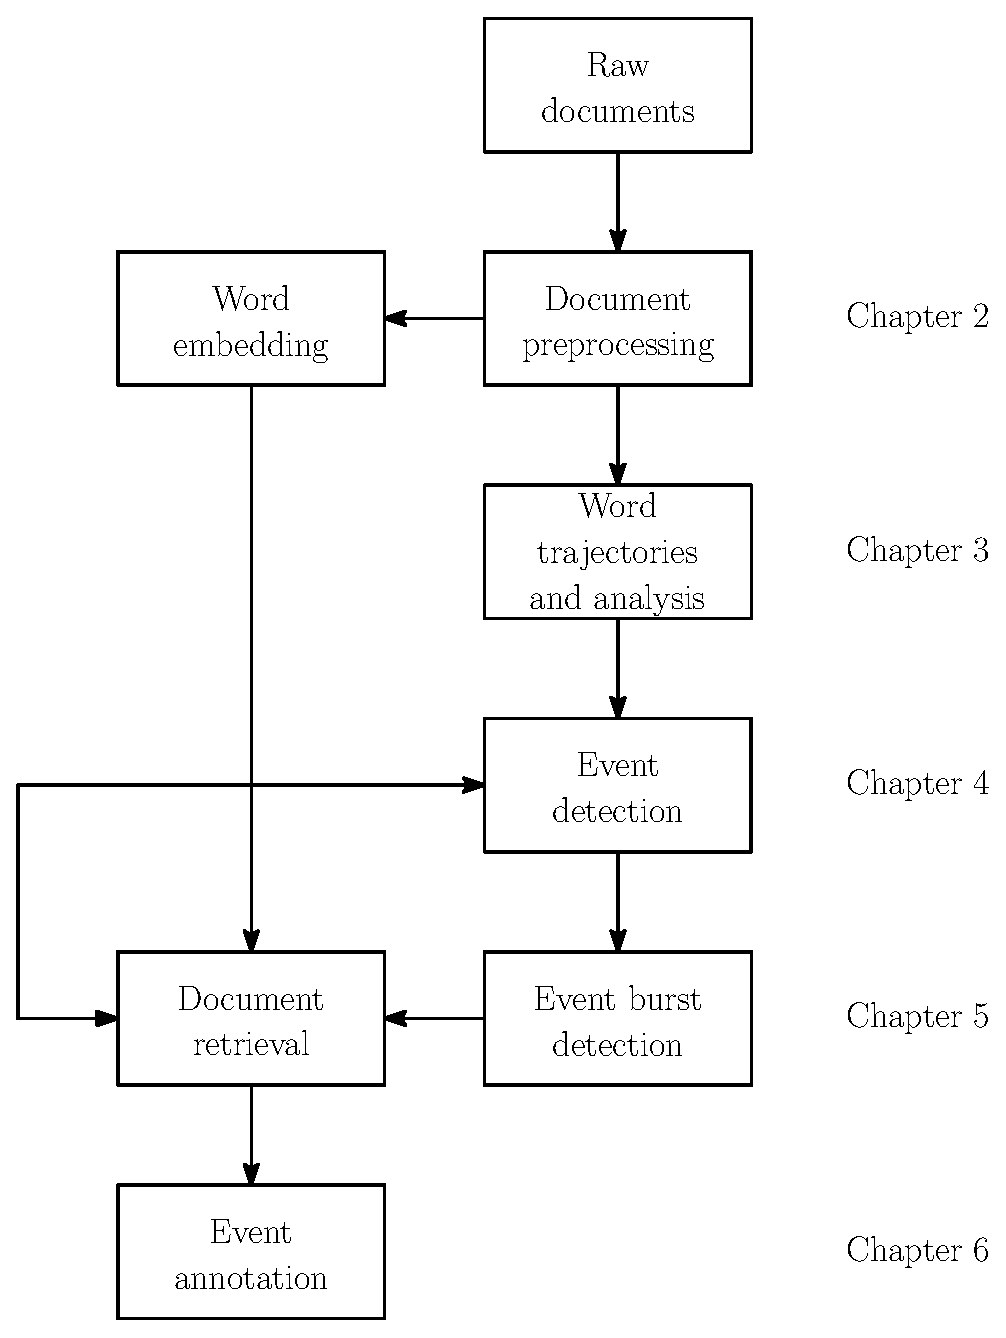
\includegraphics[height=0.6\paperheight]{diagram}
  \caption{Schematic representation of our method.}
  \label{fig:diagram}
\end{figure}